\documentclass[a4paper, 10pt]{article}

\usepackage{wrapfig}
\usepackage{listings}
%Math
\usepackage{amsmath}
\usepackage{amsfonts}
\usepackage{amssymb}
\usepackage{amsthm}
\usepackage{ulem}
\usepackage{textcomp}


%PageStyle
\usepackage[german]{babel}
\usepackage{fontenc}
\usepackage{fancyhdr, graphicx}
\usepackage{fullpage}
\usepackage{graphicx}
\usepackage{textcomp}
\usepackage{fancyhdr} %for header/footer
\usepackage{wrapfig}
%Metadata
\title{Betriebssysteme}
\author{Fabian Stebler}
\date{2. Semester (FS 2012)}


\begin{document}
\maketitle
\newpage
\section{Einleitung}
\subsection{Definition}
Ein Betriebssystem ist die Software die die Verwendung eines Computers ermöglicht. Es verwaltet Betriebsmittel wie den Speicher, die I/O-Geräte, usw.\\
\subsection{Bestandteile}
Betriebssysteme bestehen in der Regel aus einem Betriebssystemkern (englisch: Kernel), der die Hardware des Computers verwaltet, sowie grundlegenden Programmen, die dem Start des Betriebssystems und dessen Konfiguration dienen.\\
Zu den Komponenten zählen:
\begin{itemize}
\item Boot-Loader
\item Gerätetreiber
\item Systemdienste
\item Programmbibliotheken
\item Dienstprogramme
\item Anwendungen
\end{itemize}

\subsection{Varianten von Betriebssystemen}
\begin{itemize}
\item Einbenutzer- und Mehrbenutzersysteme
\item Einzelprogramm- und Mehrprogrammsysteme
\item Stapelverarbeitungs- und Dialogsysteme
\end{itemize}
Betriebssysteme finden sich in fast allen Computern: als Echtzeitbetriebssysteme auf Prozessrechnern, auf normalen PCs und als Mehrprozessorsysteme auf Hosts und Grossrechnern.

\subsection{Geschichte}
Mechanische Rechenmaschienen wurden mit der Zeit mit Lochstreifen versehen und somit konnte von einer Art Betriebssystem gesprochen werden. Später wurden die mechanischen Teile durch die Röhrentechnologie und anschliessend durch Transistoren ersetzt (ca.1947).
\begin{itemize}
\item 1955 Erfindung Mikroprogrammierung
\item 1964 Erstes modellreihenübergreifendes BS
\item 1969 Beginn Arbeit an UNIX
\item 1972-1974 Umschreiben UNIX in C (portabilität)
\item 1980-1990 Popularitätssteigerung bei Heimcomputern
\item 1981 Entwicklung erste graphische Oberfläche. Apple kauft sich mit Aktien ein, kreirt MAC und MAC OS. Verliert aber aufgrund der Experimentierfreudigkeit Marktanteile an Windows.
\item 1991 Linus Torvalds beginnt mit der Entwicklung des LINUX-Kernels. (Start Open Source Bewegung)
\item Microsoft entwickelte MS-DOS weiter und liefert MS-Windows
95 Mitte der 90‘er Jahre aus. (Tabellenkalkulation)
\item Im PC-Desktop-Bereich tobte ein eigentlicher „Glaubenskrieg“ zwischen Microsoft und Apple.
\item IBM und andere zogen sicher immer mehr in den Midrange/Mainframe-Markt zurück.
\end{itemize}

\subsection{Lessons learned}
\begin{itemize}


\item Die Grundkonzepte haben sich stark angenähert.
\item Kompatibilität wird (oft zähneknirschend) bereitgestellt.
\item Entscheide für/gegen ein Betriebssystem (bes. im Privat-
bereich) haben teilweise weltanschauliche Hintergründe.
\item Der Quellcode ist kein Geheimnis und kein Marktvorteil mehr.
\item Partizipative Entwicklung durch Communities hat ein grosses
Markt- und Sparpotential.
\item Die Positionen scheinen bezogen, der Markt wächst immer
noch stark genug, um den etablierten Anbietern Wachstum zu
ermöglichen.
\item Die Wertschöpfung hat sich verlagert:
\begin{itemize}
\item Hardware zu Betriebssystem
\item GUI zu Applikationen
\item Daten zu Business Intelligence
\end{itemize}
\end{itemize}
\newpage

\section{Blockstruktur eines Betriebssystems}
\subsection{Aufgaben des Betriebssystems}
\begin{itemize}
\item Start des Systems
\item Laden und Unterbrechen von Programmen (Laufzeitumgebung)
\item Methoden für die Interprozesskommunikation
\item Verwaltung der Prozessorzeit
\item Verwaltung des primären und sekundären Speicherplatzes für das Betriebssystem und seine Anwendungen
\item Verwaltung der angeschlossenen Geräte, Netzwerke etc.
\item Schutz des Systemkerns und seiner Ressourcen vor nicht intendierter Benutzung
\item Benutzerführung, Rollen und Rechte
\item Einheitliche Schnittstelle für die System- und Anwendungsprogrammierung Ereignisprotokollierung

\end{itemize}

\subsection{Grapische Darstellung}
Untenstehende Grafik zeigt die Schichtenarchitektur eines modernen Betriebssystems (Linux).\\
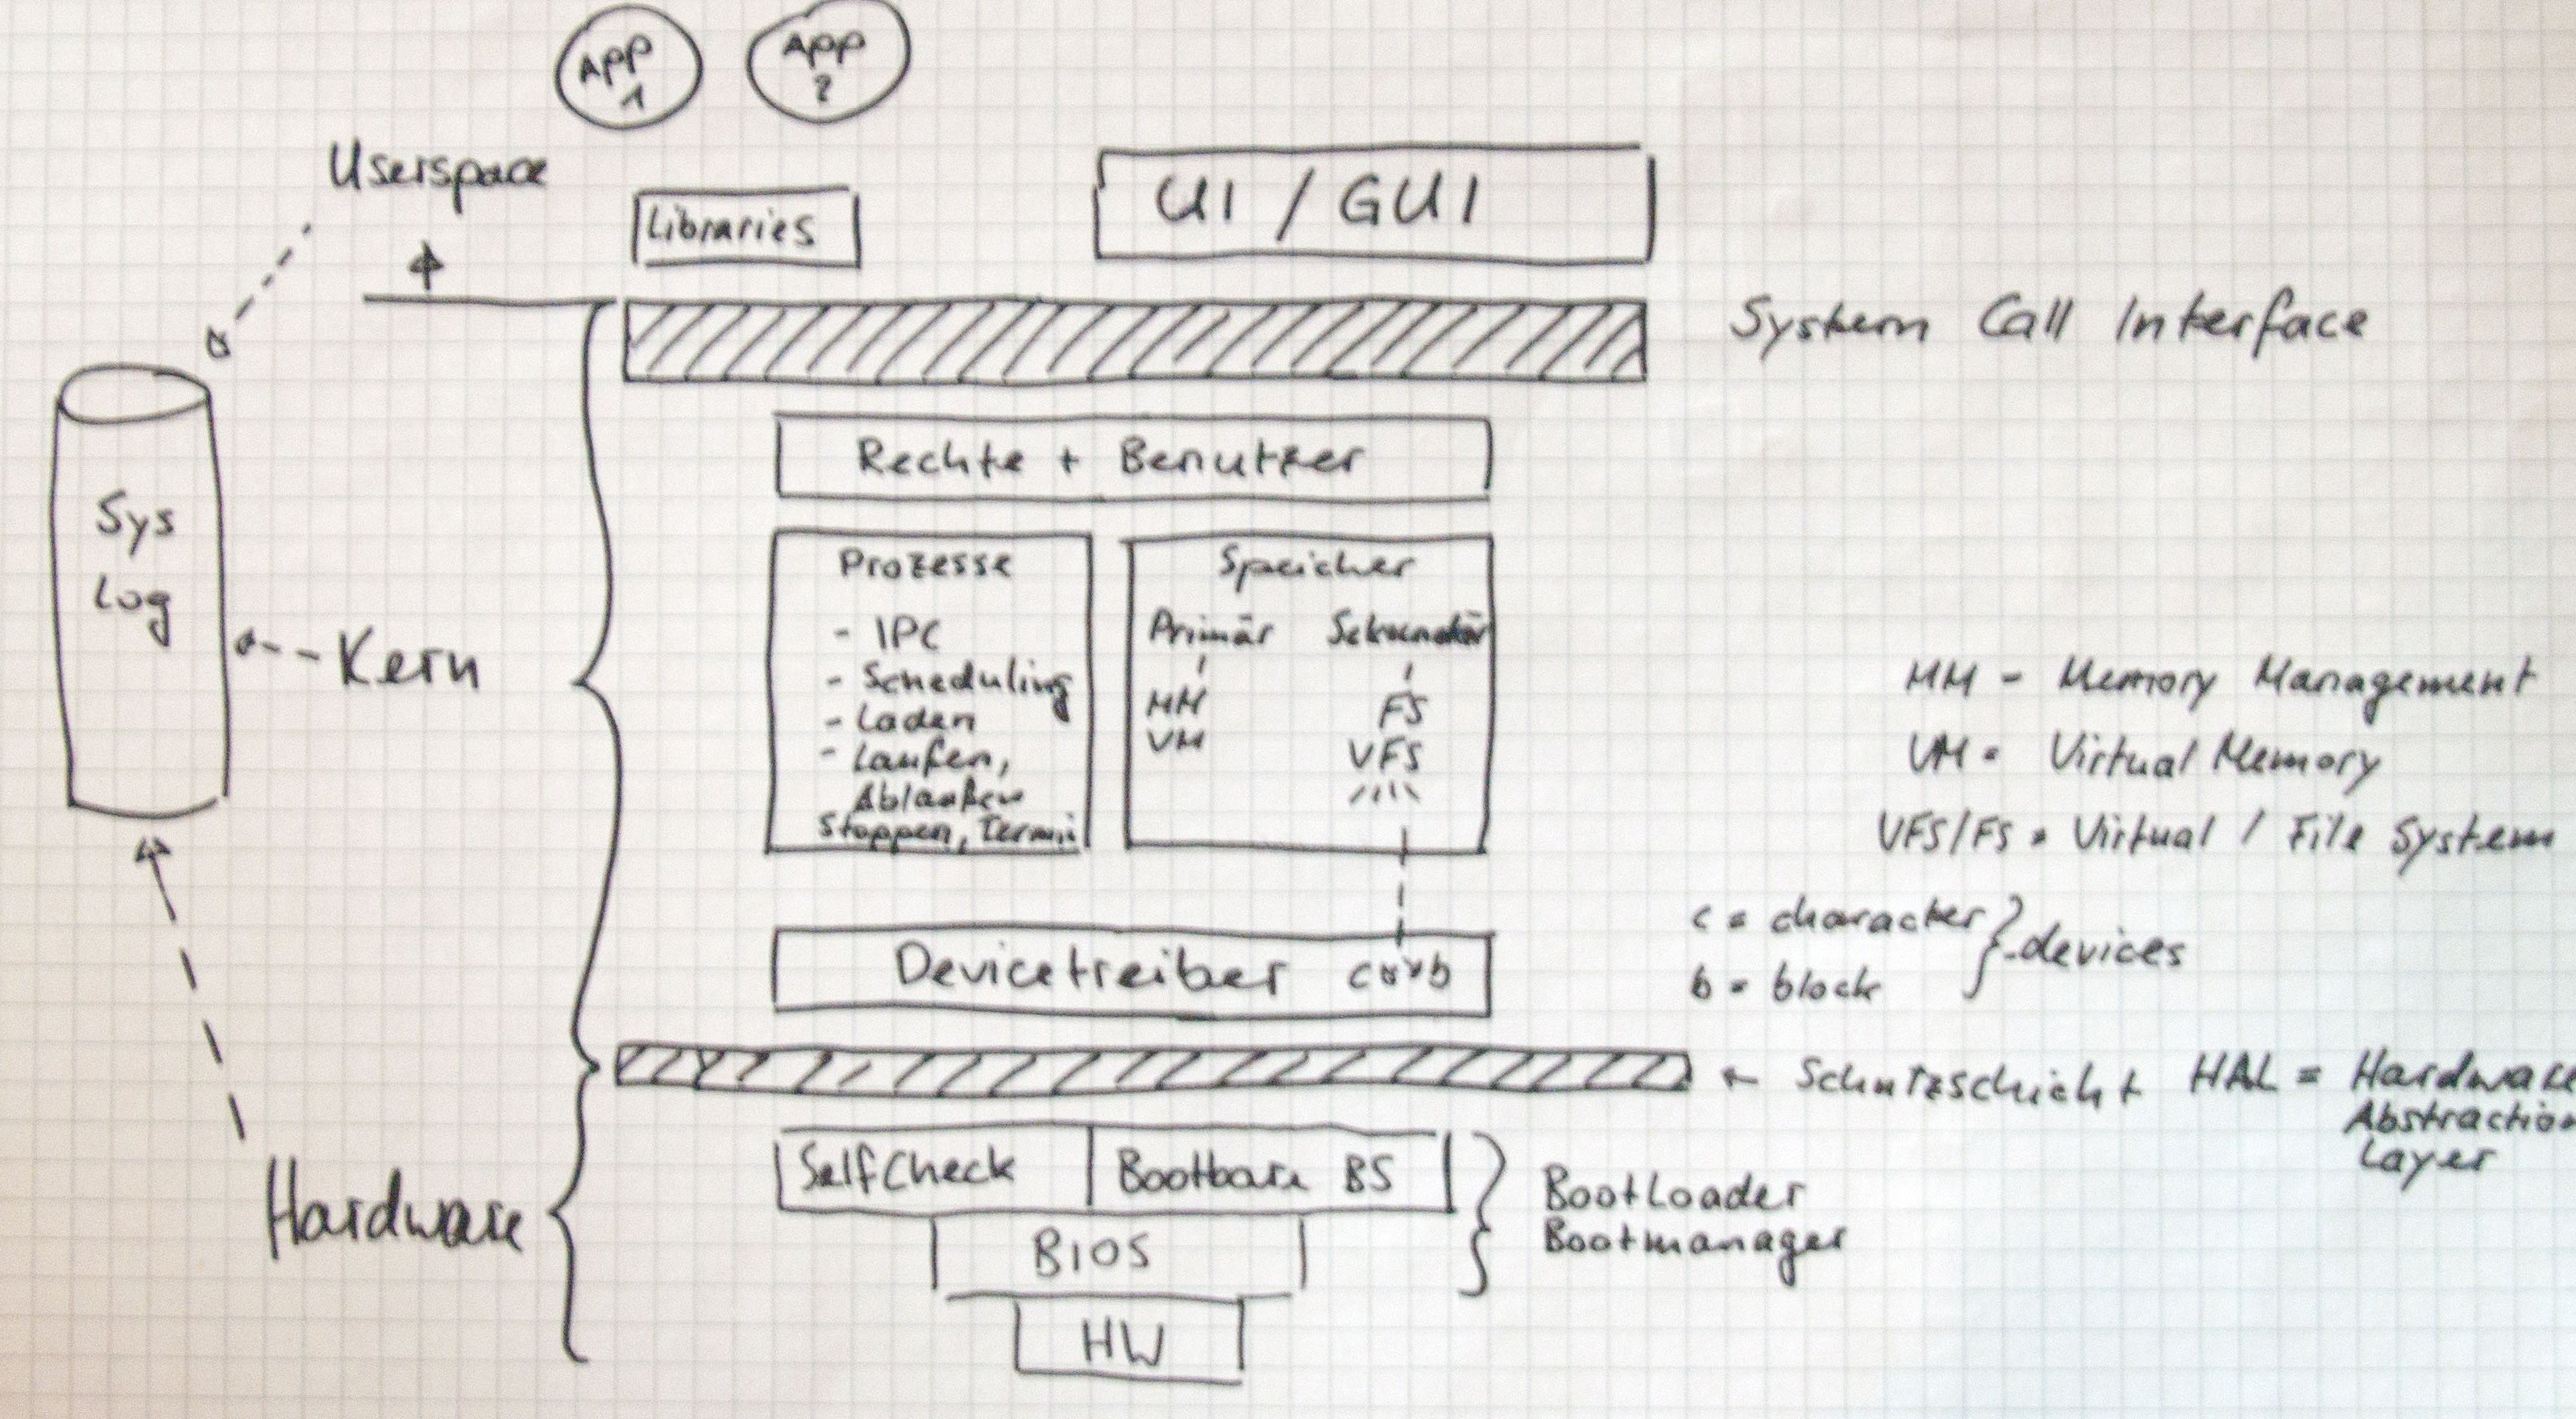
\includegraphics[scale=0.15]{Bsys.jpg}\\

\subsection{Aufgabenteilung der Blöcke}
\subsubsection{Dateisystem}
\begin{itemize}
\item Struktur des Dateisystems (Baum, Graph, flach, ...)
\item Strukturelemente (Directories)
\item Zugriffsrechte auf Directories und Dateien
\item Anlage, Suche, Manipulation, Löschen von Dateien
\item Verwaltung von Datenblöcken auf Speichermedien
\item Kombination von Dateisystemen (mounting)
\item Benutzerschnittstelle und Navigation
\item Backup / Restore
\end{itemize}

\subsubsection{Prozesssteuersystem}
\begin{itemize}
\item Prozesse kreieren
\item Prozesse starten
\item Prozesse schedulen, Warteschlangen, Ressourcenverbrauch
\item Prozesse stoppen / unterbrechen
\item Prozesse terminieren (freiwillig / wegen Fehler)
\item Prozesskommunikation (Prozess-Prozess und Kern-Prozess / Prozess-Kern)
\item Zuordnung von Hauptspeicher und anderen geteilten Ressourcen
\item Ein-/Auslagerung von Prozessen
\item Prozesse und ihre Zustände anzeigen
\end{itemize}

\subsubsection{System Call Interface}
\begin{itemize}
\item Einzige Schnittstelle zwischen Kern und Benutzer
\item Normierung der Syntax und Semantik (POSIX 1003)
\item Parametrisierung und Übergabe
\item Übergabe der Kontrolle $\rightarrowtail$ Betriebsmodi
\end{itemize}

\subsubsection{Programmierung}
\begin{itemize}
\item Wahl der Programmiersprache / Systempräferenz
\item System-/Applikationsnahe Bibliotheksfunktionen
\item Programmierumgebung (Editor, Compiler, Assembler, Linker, Loader, Debugger)
\item „Bundling“ in einer Applikation (z.B. Eclipse)
\end{itemize}

\subsubsection{Benutzerschnittstelle}
\begin{itemize}
\item Textuelle Basis-Schnittstelle mit Kommando-Interpreter (Shell) Konsole
\item Programmierbarkeit (Scripting, Pipelining, I/O-Redirection) der Benutzerschnittstelle
\item Graphische Benutzerschnittstelle (GUI) mit
\item Abstraktion der unterliegenden Komplexität und Syntax für Nicht Systemspezialisten
\item Austauschbarkeit der Shell und der Systembefehle (Applikationen)
\end{itemize}


\subsubsection{I/O Management}
Ein Betriebssystem muss auch die Hardware kontrollieren:
\begin{itemize}
\item Die Fähigkeiten der Hardware voll ausschöpfen.
\item Die verschiedenen inhomogenen Komponenten zu einer Einheit formen.
\item Die Hardware schützen vor unerlaubtem Zugriff.
\end{itemize}
Anm.: Peripheriegeräte sind meist unterschiedlich, sollten aber leicht in das System integrierbar sein.

\subsubsection{File System als generelle Schnittstelle}
Die Idee von Unix war, dass File System für möglichst viele Subsysteme als Schnittstelle zu verwenden.
\begin{itemize}
\item Dateien, Directories
\item Prozesssynchronisation (Lock Files, ...)
\item Prozesskommunikation (Pipes, Sockets)
\item Peripheriegeräte (Device Special Files)
\item Kommunikationsprotokolle (TCP/IP, ...)
\item Prozesse (/proc Dateisystem)
\end{itemize}
Anm.: Es bedingt einer zusätzlichen Abstraktionsschicht.

\newpage
\section{Filesystem}
Die anschliessende Graphik zeigt ein virtuelles Dateisytem:\\
\\
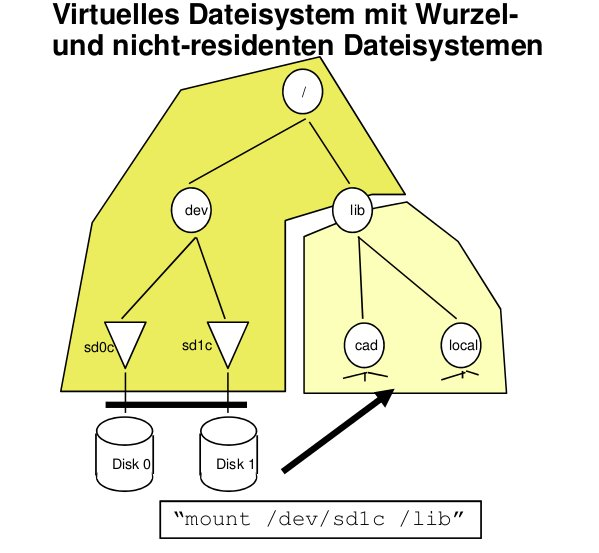
\includegraphics[scale=0.4]{Dateisystem.jpg}\\

\subsection{Partition auf der Disk}
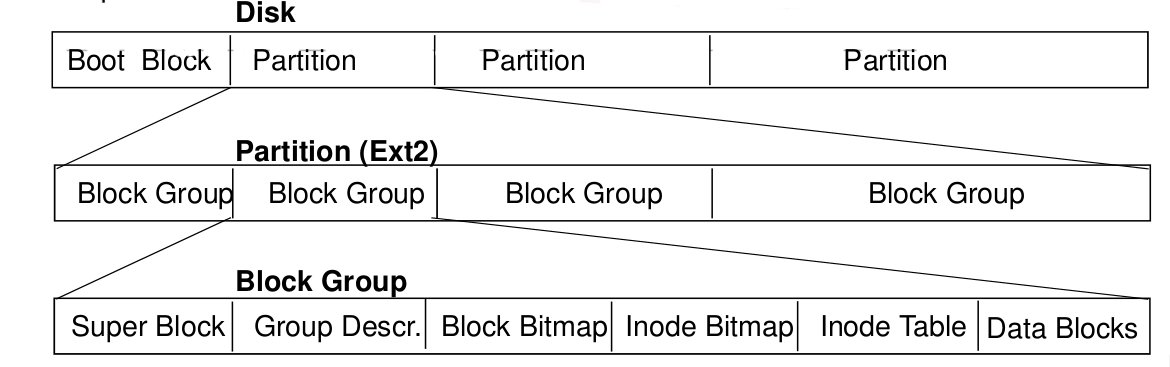
\includegraphics[scale=0.3]{Partition_HD.jpg}\\
\\
Superblockinhalt:
\begin{itemize}
\item Anzahl inodes und Datenblöcke
\item Adresse des 1. Datenblocks
\item Anzahl freie Blöcke und inodes
\item Grösse eines Datenblocks
\item Blöcke / inodes pro Gruppe
\item Anzahl Bytes pro inode
\end{itemize}

\subsection{Blockallokationen}
\subsubsection{Zusammenhängende Belegung}
Vorteile:
\begin{itemize}
\item Einfachste aller Methoden
\item Sehr schneller direkter Zugriff auf die Daten
\item Für die Lokalisierung der Dateiblöcke brauchen wir
nur Anfangsblock und Größe der Datei zu wissen.
\item Lese-Operationen können sehr effizient implementiert
werden.
\item Gute Fehlereingrenzung
\end{itemize}
Nachteile:
\begin{itemize}
\item Dynamische Dateigrößen sind ein Problem
\item Im Laufe der Zeit wird die Platte fragmentiert.
\item Platz zu finden für neue Dateien ist ein Problem
\item Verwaltung von freien Speicherplätzen notwendig
\item Regelmäßige Kompaktifizierung notwendig
\item Platte hin- und zurück kopieren
\end{itemize}
\subsubsection{Verlinkte Blöcke}
Jede Datei wird als verkettete Liste von Plattenblöcken gespeichert. Nur die Plattenadresse des ersten und letzten Blocks wird in dem Verzeichniseintrag gespeichert.\\
Vorteile:
\begin{itemize}
\item Keine externe Fragmentierung
\item Sequenzieller Zugriff ist kein Problem
\end{itemize}
Nachteile:
\begin{itemize}
\item Schlechter wahlfreier Zugriff auf Dateiinhalte
\item Jeder Verweis verursacht einen neuen Plattenzugriff
\item Overhead für das Speichern der Verkettung (Lösung: clusters aus mehren Blöcken)
\item Erhöhter Aufwand bei Dateizugriffen
\item Schlechte Fehlereingrenzung
\end{itemize}

\subsubsection{Filemap (Landkarte)}
\begin{wrapfigure}{r}{8cm}
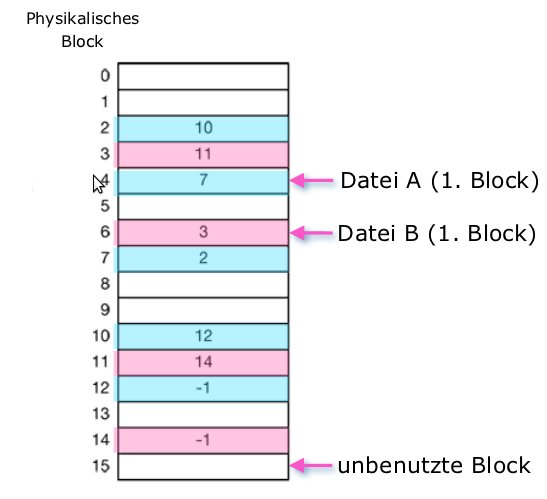
\includegraphics[scale=0.4]{filemap.jpg}
\end{wrapfigure}

Vorteile:
\begin{itemize}
\item Dateien können sehr leicht und effizient vergrößert werden
\end{itemize}
Nachteile:
\begin{itemize}
\item Interne Fragmentierung
\item schlecht für random accesses
\item fehleranfällig
\end{itemize}
\newpage
\subsubsection{Index Allokation}
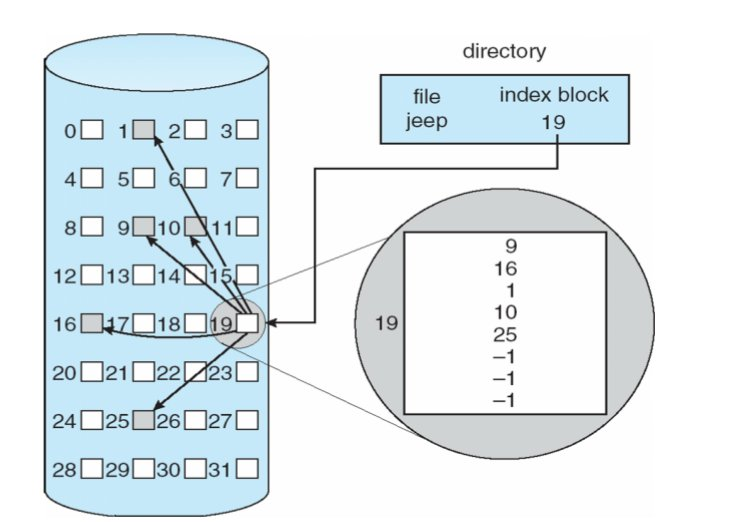
\includegraphics[scale=0.5]{index_allocation.jpg}

\subsection{Struktur von Inodes}
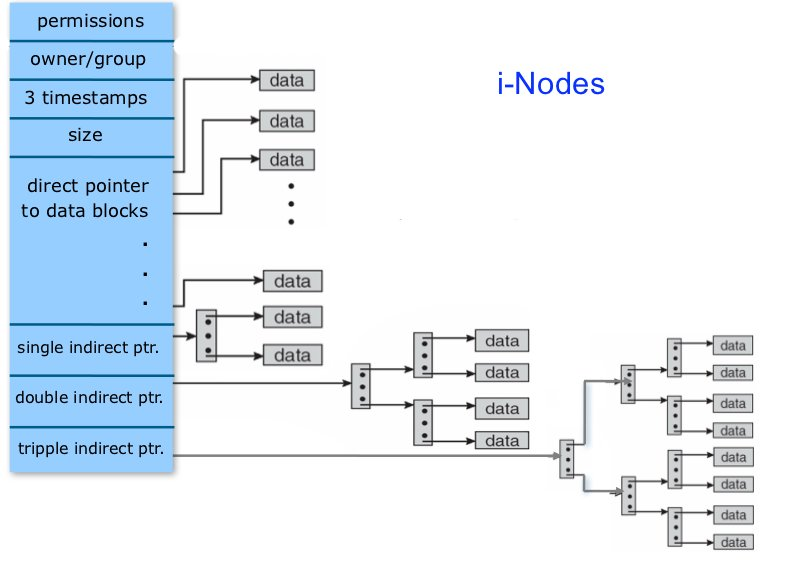
\includegraphics[scale=0.6]{inodes.jpg}

\subsubsection{Informatione Inode}
\begin{tabular}{p{7cm}|p{7cm}}
\textbf{Auf der Disk} & \textbf{Zusätzlich im Memory} \\ \hline
\begin{itemize}
\item Inode Nummer
\item Anzahl hard links
\item Typ (-, l, d, b, c, p)
\item Rechte (-, r, w, x, s)
\item Besitzer
\item Gruppe
\item Grösse
\item Letzte “access time”
\item Letzte “content change time”
\item Letzte “inode modification time”
\item Datenblock Information
\end{itemize}
&
\begin{itemize}
\item Link auf die “hash list”
\item Link auf die “inode list”
\item Benutzerzähler
\item Gerätenummer
\item “Device special file” Indikator
\item Grösse eines Blocks
\item Anzahl Blöcke
\item Lock auf den inode
\item “Mount point” Indikator
\item Warteschlange wartender Prozesse
\item Locks auf die Datei
\item Hauptspeicher-Region (für Memory-mapped file I/O)
\item Belegte Seiten im Hauptspeicher
\end{itemize}
\end{tabular}

\subsection{Designvorgaben für Filesystem}
\begin{itemize}
\item Anzahl Disks und Disk Controller
\item Verteilung auf Partitionen
\item Blockgrösse pro Partition
\begin{itemize}
\item Grosse Blöcke: schneller Zugriff auf Dateien (Datei-Durchschnittsgrösse $<$ 4 kB)
\item Kleine Blöcke: weniger interne Fragmentierung
\end{itemize}
\item Anzahl Dateien / Inodes pro Partition
\begin{itemize}
\item Wenige Inodes: mehr Platz für Dateiblöcke
\item Viele Inodes: mehr Dateien pro Partition mgl.
\end{itemize}
\end{itemize}

\newpage
\section{Prozesse}

\subsection{Einleitung}

\subsubsection{Was ist ein Prozess?}
Ein oder mehrere Programme (deterministische Sequenz von Instruktionen) werden auf einem oder mehreren physischen oder virtuellen Prozessoren ausgeführt. Zu jedem Zeitpunkt der Ausführung verbunden mit einem “computational state” (aktuell verwendete Variablen etc. im Programm), externe Ressourcen wie Zustand der CPU, Register, Zeitnahme, usw. Ein Prozess wird durch das Betriebssystem strikt überwacht und verwaltet

\subsubsection{Anforderungen an ein Prozess-Steuersystem}
\begin{itemize}
	\item Prozesse kreieren
	\item Prozesse starten
	\item Prozesse schedulen, Warteschlangen, Ressourcenverbrauch
	\item Prozesse stoppen / unterbrechen
	\item Prozesse terminieren (freiwillig / wegen Fehler)
	\item Prozess-Signalisierung und -kommunikation
	\item Faire Zuordnung von Hauptspeicher und anderen geteilten Ressourcen
	\item Ein-/Auslagerung von Prozessen bei vollem Speicher
	\item Prozesse und ihre Zustände anzeigen
\end{itemize}

\subsubsection{Unix-Prozess Segmente}
\begin{itemize}
	\item Text Segment (8 K)
	\item Daten Segment (32 K)
	\item Stack Segment (64 K)
	\item Shared Memory Segment
	\item Mapped File Segment
\end{itemize}

\subsection{Kernel und User Mode}
Ein Prozess hat mindestens (in Unix genau) zwei Ausführungsmodi:
\begin{description}
	\item[User Mode:] Es wird der normale Programmcode ausgeführt.
	\item[Kernel Mode:] Ss werden Systemaufrufe ausgeführt oder Ausnahmen behandelt.
\end{description}
Der Übergang erfolgt durch einen Systemaufruf durch das Programm, eine Ausnahmesituation (Fehler) oder durch asynchrone Events (Kom- munikation etc). Beide Modi haben separate Segmente und sind voneinander abgeschirmt.

\subsubsection{Prozess-/Kontext- Wechsel}
Wenn ein Prozess:
\begin{itemize}
	\item warten muss (z.B. auf I/O oder einen Event),
	\item seine zugeordnete Laufzeit oder andere Ressourcen- grenzen erreicht bzw. überschreitet,
	\item terminiert oder gestoppt wird,
	\item die CPU freiwillig abgibt
\end{itemize}
muss das Betriebssystem die CPU einen anderen ablaufbereiten Prozess zuteilen und diesen starten. Dies erfordert das Abspeichern des exakten Prozess- Zustandes und das spätere Restaurieren, wenn der Prozess wieder weiterlaufen soll.\\

\begin{wrapfigure}{r}{7cm}
\includegraphics[scale=0.2]{process_region_table.png}
\end{wrapfigure}

\subsubsection{Kernel-Datenstrukturen für das Prozess-Management}
In älteren Unix-Varianten ist die Grösse der Prozesstabelle statisch (schnelle Indexierung, Lizenzierung über Anzahl Prozesse / Benutzer).\\
Alternativ kann die Prozesstabelle eine verkettete Liste sein (variable Anzahl Prozesse, aber komplizierte Indexierung und Überlauf-Gefahr). \\
Linux verwendet eine Mischform (dynamisch angelegte Prozesskon- trollblöcke (PCB) in einer verketteten Liste mit einer statischen Hash- Tabelle für die schnelle Suche).

\subsection{Sichern des Prozess Kontexts}
\includegraphics[scale=0.3]{save_process_context.png}

\subsection{Prozess Zustände}
\includegraphics[scale=0.5]{process_states.png}

\subsection{Prozess-bezogene System Calls}
\begin{description}
	\item[fork] Erstellen eines neuen Prozesses durch Kopieren
	\item[exec] AusführeneinesneuenProgrammsineiner vorhandenen Prozesshülle
	\item[Signal] Stoppen eines Prozesses
	\item[exit] Terminieren eines Prozesses
	\item[wait] Warten auf das Terminieren eines Prozesses, einfache Synchronisation
\end{description}

\subsection{Prozesse versus Threads}
Kontextwechsel sind eine “schwere” Operation mit viel Verarbeitungsaufwand durch den Kernel. Da viele Unix-Prozesse I/O-intensiv sind, verbringen sie die meiste Laufzeit mit Warten, dadurch erhöht sich die Anzahl von Kontextwechseln im System. Neuere Unix-/Linux-Systeme unterstützen mehr als einen parallelen Ausführungspfad innerhalb eines Prozesses (multi-threading). Es muss kein Kontextwechsel vorgenommen werden, um eine andere Aktivität zu starten. \\
Aber:
\begin{itemize}
	\item Das Scheduling muss innerhalb des Prozesses erfolgen,
	\item die Threads sind verwandt, d.h. ihr Code liegt innerhalb des gleichen Unix-Prozesses,
	\item der Programmierer muss für die Datenintegrität selbst sorgen.
\end{itemize}
\includegraphics[scale=0.3]{process_vs_threads.png}

\subsubsection{Basismodell für Threads}
\begin{itemize}
	\item Kernel-Code (System Call Interface) oder Library?
	\item Ausführungsmodelle
		\begin{itemize}
			\item Master/Slave(s)
			\item Cooperating Pool
			\item Pipeline
			\item Hybrid
		\end{itemize}
	\item Besondere Anforderungen
		\begin{itemize}
			\item Synchronisation
			\item Betriebsmittel-Zuteilung (Scheduling)
			\item Ausnahmebehandlung
		\end{itemize}
\end{itemize}

\subsubsection{Benutzungs- und Administrationssicht auf ein Prozess-Steuersystem}
\begin{itemize}
	\item Prozess-Erzeugung und –Termination
	\item Identifikation
	\item Priorisierung
	\item Besitzer	
	\item Ressourcenverbrauch
	\item Prozess-Ein-/Auslagerung
	\item Signalisierung
	\item Prozesskommunikation
\end{itemize}

\newpage
\section{I/O, Peripherie}
\subsection{Anforderungen von Peripheriegeräten}
\begin{itemize}
	\item Ressourcenverwaltung:
		\begin{itemize}
			\item Hauptspeicher für Zwischenpufferung von Daten beim Transfer
			\item CPU-Zeit für das Behandeln asynchroner Events (z.B. Ankunft von Daten an der Netzwerkschnittstelle)
		\end{itemize}
	\item Zugriffssteuerung und –synchronisation:
		\begin{itemize}
			\item Einheitliche Schnittstelle
			\item Synchronisation von Zugriffen durch die Prozesse
			\item Signalisierung
		\end{itemize}
	\item Scheduling
\end{itemize}

\subsection{Aufgaben und Funktionsweise des I/O-Subsystems}
\begin{itemize}
	\item Aufgabe: schneller und zuverlässiger Datentransfer zwischen Geräten (Disk, Drucker, Tastatur, Bildschirm, Maus etc.) und Prozessen, d.h. Datenstrukturen im Prozess-Adressraum (read und write Operationen)
	\item Design: Das I/O Subsystem besteht aus einer oberen Schicht, die Daten zwischen dem Benutzer- und dem Kernel-Adressraum bewegt, und einer unteren Schicht, die Daten zwischen dem Kernel-Adressraum und den Geräten bewegt.
	\item Standardisiertes I/O (Geräteunabhängigkeit bezüglich Programmierung und Benutzung)
	\item Optimiertes I/O (abhängig vom Gerät und dessen Eigenschaften, Durch- satz, Sicherheit usw.)
	\item Konsistenz trotz Unterbrechbarkeit der Operationen und Zugriffssicher- heit wenn Daten zwichen Kernel und Benutzer-Prozess bewegt werden
	\item Drei Typen von I/O: Datei-basiert, Zeichen-basiert, STREAM-basiert
\end{itemize}

\subsection{Buffer-Cache}
\subsubsection{Der klassische Buffer Cache}
\begin{itemize}
	\item Ziel: Optimierung des Zugriffs auf block-orientierte geräte, maximale Menge Daten im Speicher behalten.
	\item Strategie 1: vorausschauendes Lesen (read ahead)
		\begin{itemize}
			\item Vorteil: beschleunigt das sequentielle Lesen (z.B. einer Datei)
			\item Risiko: potentielle Verschwendung von Hauptspeicher
		\end{itemize}
	\item Strategie 2: verzögertes Schreiben (delayed write)
		\begin{itemize}
			\item Vorteil: Bündeln von Daten in Blöcke für das Schreiben auf langsame Geräte (z.B. Disk)
			\item Risiko:nacheinemerfolgreichenwrite()Systemaufrufsind die Daten noch nicht auf der Disk gespeichert (Verlustrisiko)
		\end{itemize}
	\item Optimiert für die Arbeit mit dummen Peripheriegeräten
\end{itemize}


\section{Hauptspeicherverwaltung}
\subsection{Virtual Memory}
\begin{itemize}
\item Hauptspeichererweiterung pro einzelnes System oder Prozess.
\item Systematische Abstraktion für systemspezifische Overlay-
Techniken
\item Organisation des Hauptspeichers in gleich grosse,
einheitlich adressierbare Einheiten (Seiten, pages)
\item Benötigt hardware-unterstütze Abbildung zwischen
physischen und virtuellen Adressen
\end{itemize}

\subsection{Swapping}
Swapper (Process 0) wird periodisch vom Kernel aufgerufen.\\

Swap Device  $\longleftrightarrow$ Swapper $\longleftrightarrow$ Hauptspeicher\\

Swap Out (Hauptspeicher zu SwapDevice):
\begin{itemize}
\item Kein Platz im HS für weitere Prozesse, Prozess ruft aber fork auf $\Rightarrow$ fork swap
\item Kein Platz im HS aber Prozess wächst, weil z.B. Stack wächst $\Rightarrow$ expansion swap
\item Swap Device ausgelagerter wartender Prozess wird ready to run und wird vom Scheduler ausgeführt $\Rightarrow$ exchange swap
\end{itemize}

Swap In (SwapDevice zu Hauptspeicher):
\begin{itemize}
\item Nur ready to run Prozesse sind wählbar $\Rightarrow$
\item Präferenz auf Prozesse die > 2 sec. Ausgelagert waren
\end{itemize}

\subsection{Demand Paging}
Anforderung: ein einzelner Prozess soll grösser sein dürfen, als der
verfügbare Hauptspeicher.\\
\\
Voraussetzungen:
\begin{itemize}
\item Hardware unterstützt seitenorientieres Speichermanagement (1$/$2 $–$ 4 kB / Seite)
\item Wiederaufsetzbare CPU-Instruktionen (wenn Instruktionen über eine Seiten-
grenze verlaufen)
\end{itemize}

Idee:\\
Nur die gerade verwendeten Teile des Codes werden geladen. Dies sind 10 bis 15 
Prozent die im HS liegen (working set). Wird auf eine Seite zugegriffen die nicht geladen ist, so gibt es einen page fault und die Seite wird nachgeladen.\\

Optimierung des “demand paging” durch
\begin{itemize}
\item Reference bit $\rightarrow$ ermöglicht nicht-lineares “working set”
\item Age bit $\rightarrow$ verbleibende Zet einer Seite im “working set”
\end{itemize}
Zwei Aufgaben für das Paging-Subsystem:
\begin{itemize}
\item Seitenalterung und Auslagerung/Löschung genügend alter Seiten
\item Bearbeitung von “page faults”
\end{itemize}

\section{Sheduling Strategien}
Funktionsweise:
\begin{itemize}
\item Fairness / Regeleinhaltung bezüglich der Zuteilung von Betriebsmitteln an Prozesse gemäss definierter Kriterien
\item Vermeidung von „Starvation“ und „Deadlocks“
\end{itemize}
Einsatzgebiete:
\begin{itemize}
\item Echtzeitsysteme mit „harten“ Garantien
\item Möglichst unterbruchsfreie Batchverarbeitung
\item Interaktives Mehrbenutzersystem
\end{itemize}

\subsection{Scheduling in Unix}
3 Prioritätsklassen:
\begin{itemize}
\item Realtime: Scheduling mit fixen Prioritäten
\item System: Geschlossene Scheduling-Klasse für Systemprozesse
\item Time-Shared: Für alle Benutzerprozesse
\end{itemize}

Prioritäts-basiertes Scheduling:
\begin{itemize}
\item Verminderte Prozesspriorität mit steigendem Ressourcenverbrauch
\item Verminderung der Priorität gemäss Laufzeit
\end{itemize}
Scheduling-Strategien:
\begin{itemize}
\item Kleine, schnelle Prozesse präferieren (z.B. Shell)
\item Ressourcen-intensiven Prozessen alle benötigten Ressourcen geben:
Schnellere Beendigung und Freigabe und Beendigung im Zeitlimit
\end{itemize}


\section{Systemüberwachung}
Was kann alles sinnvollerweise Überwacht werden:
\begin{itemize}
\item Betriebssystem Typ, Alter
\item Laufzeitüberwachung
\item Verschiedene Speicher, Prozesse CPU, RAM, Disks
\item Auslastung/Trending CPU
\item Netzwerkanschlüsse
\item Autorisierter Anschluss an Netzwerk
\item Peripheriegeräte, 
\item Backupüberwachung
\item Software und Version, Lizenz
\item Laufzeitüberwachung Disk
\item Benutzer und Berechtigung
\end{itemize}

Anm.: Verschiedene Fachbegriffe rund um Systemüberwachung
\begin{itemize}
\item Incident (Einzelfall)
\item Problem (Reihung)
\item Desaster (Notfallplan ausführen!)
\item Triage (Rollen, Verantwortlichkeiten, Beurteilungskriterien, Prozesse, Zeitfaktor, ...)
\end{itemize}


\end{document}